% This section breaks down your layer abstraction to another level of detail. Here you grapically represent the logical subsytems that compose each layer and show the interactions/interfaces between those subsystems. A subsystem can be thought of as a programming unit that implements one of the major functions of the layer. It, therefore, has data elements that serve as source/sinks for other subsystems. The logical data elements that flow between subsystems need to be explicitly defined at this point, beginning with a data flow-like diagram based on the block diagram.

Figure 3 describes the layers that the Checkers-playing co-bot comprises of and the subsystems that make up each layer. 

The Computer layer, Move Decision layer, Move Execution layer, and External Components layer have subsystems within their layers. While these layers interface each other, the subsystems within them also interface with each other. Within the Computer layer, the software works with both the HUD and GUI to implement the user interface. Within the Move Decision layer, the computer vision component communicates with the AI to train and interpret information that is being captured by the camera. Within the Move Execution layer, the Arduino controller powers and instructs the magnetic gripper when it needs to be activated and deactivated. Within the External Components layer, the checkers pieces are manipulated across the playing board and disposed into the collection box.

As a whole, the Computer layer communicates with the opponent layer, the Move Decision layer, the Move Execution layer, and the input button/device layer. This is because the robot control system is a part of the software and the opponent interacts with the information displayed by the GUI. The Opponent layer also interfaces with the input button layer and External Components layer when it is their turn during the match. The Move Execution layer also interfaces with the External Components layer during the match. The Move Decision layer and the External Components layer interfaces with the camera where it captures the state of the game board and communicates it to the CV and AI components for data interpretation.  

\begin{figure}[h!]
	\centering
    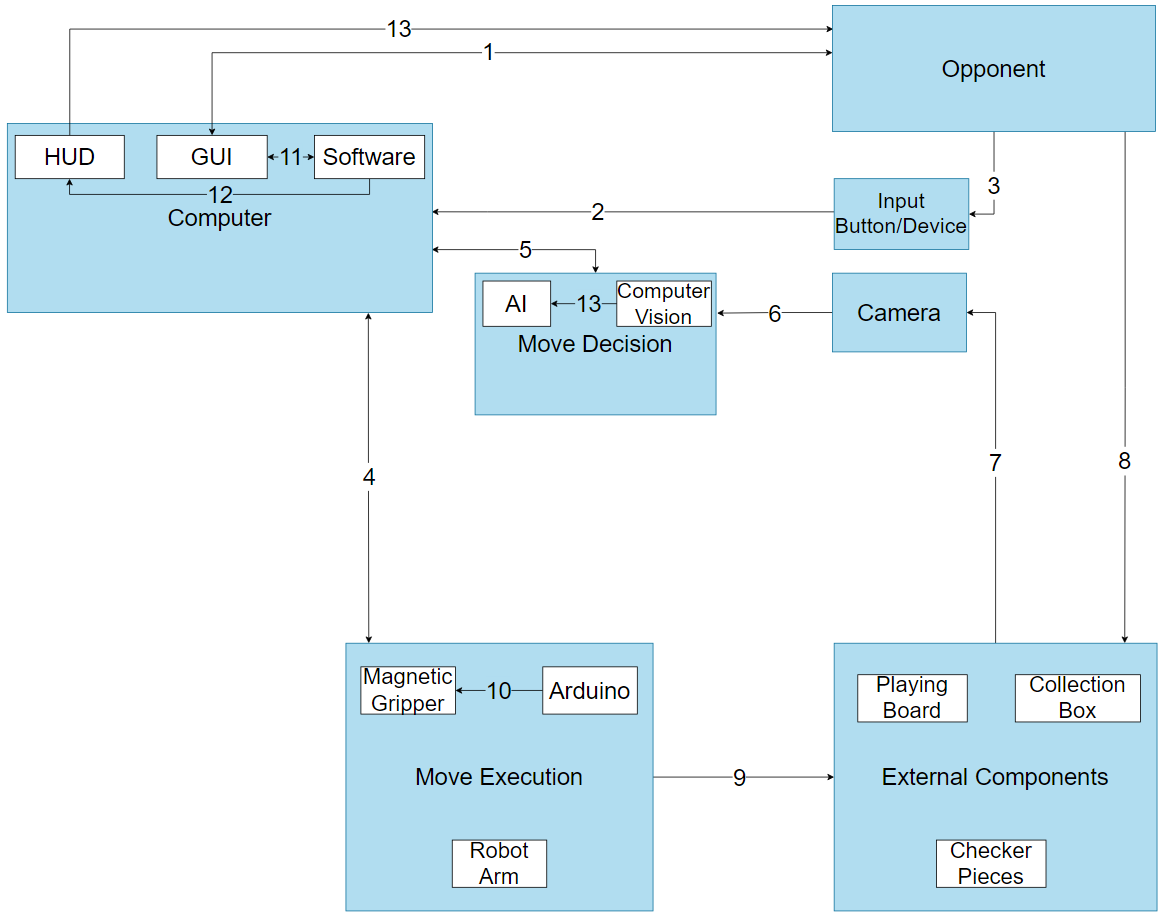
\includegraphics[width=0.90\textwidth]{images/data_flow_actual.png}
 \caption{Checkers-Playing UR5 Co-bot architectural layer diagram}
\end{figure}
